\section{MongoDB}
\subsection{Giới thiệu về MongoDB}
\begin{enumerate}
    \item Định nghĩa:
    \item []\hspace*{0.7cm} MongoDB là một chương trình quản lý cơ sở dữ liệu NoSQL mã nguồn mở. NoSQL (Không chỉ SQL) được sử dụng thay thế cho cơ sở dữ liệu quan hệ truyền thống. Cơ sở dữ liệu NoSQL khá hữu ích để làm việc với các bộ dữ liệu phân tán lớn. MongoDB là một công cụ có thể quản lý thông tin định hướng tài liệu, lưu trữ hoặc truy xuất thông tin.\cite{noauthor_what_nodate_dn_DB}
    
    \item Lịch sử phát triển:
    \item []\hspace*{0.7cm}MongoDB được bắt đầu phát triển vào đầu năm 2007 khi công ty 10gen đang phát triển một nền tảng tương tự dịch vụ Azure\footnote{Microsoft Azure là nền tảng điện toán đám mây của Microsoft, cung cấp các dịch vụ như cơ sở hạ tầng (IaaS), nền tảng (PaaS) và phần mềm (SaaS). Azure cho phép doanh nghiệp phát triển, triển khai và quản lý ứng dụng mà không cần quản lý cơ sở hạ tầng. Nền tảng này nổi bật với khả năng mở rộng, chi phí hiệu quả và tích hợp dễ dàng với các sản phẩm khác của Microsoft. Azure cũng cung cấp các dịch vụ phân tích, trí tuệ nhân tạo, và bảo mật để hỗ trợ doanh nghiệp trong việc tối ưu hóa hoạt động và bảo vệ dữ liệu.} của Microsoft. Công ty 10gen là một công ty phần mềm có trụ sở tại New York, nay được đổi tên thành MongoDB Inc. Việc phát triển ban đầu tập trung vào xây dựng PaaS (một nền tảng dịch vụ) nhưng sau đó vào năm 2009, MongoDB đã xuất hiện trên thị trường như một dự án mã nguồn mở máy chủ cơ sở dữ liệu và được duy trì bởi chính tổ chức này.\cite{noauthor_mongodb_2023} 
    
    \item []\hspace*{0.7cm}Tháng 3 năm 2010, MongoDB Inc. đã tung ra sản phẩm sẵn sàng đầu tiên của mình là phiên bản 1.4. Phiên bản ổn định tiếp theo của MongoDB là phiên bản 2.4.9 được phát hành vào ngày 10 tháng 1 năm 2014.
    \item []\hspace*{0.7cm}Đầu năm 2015, phiên bản 3.0 được phát hành, cuối năm 2015 phiên 3.2 ra đời đi kèm với công cụ quản trị trên giao diện đồ họa MongoDB Compass.
\end{enumerate}

\subsection{Cách MongoDB hoạt động}
\begin{enumerate}
    \item []\hspace*{0.7cm}MongoDB hoạt động dưới dạng một hệ thống cơ sở dữ liệu phi quan hệ, lưu trữ dữ liệu dưới dạng tài liệu (document) JSON. Dữ liệu được lưu trữ trong collections và documents. Do đó, database, collection và documents sẽ có liên quan với nhau như hình dưới đây:
    \begin{figure}[h]
        \centering
        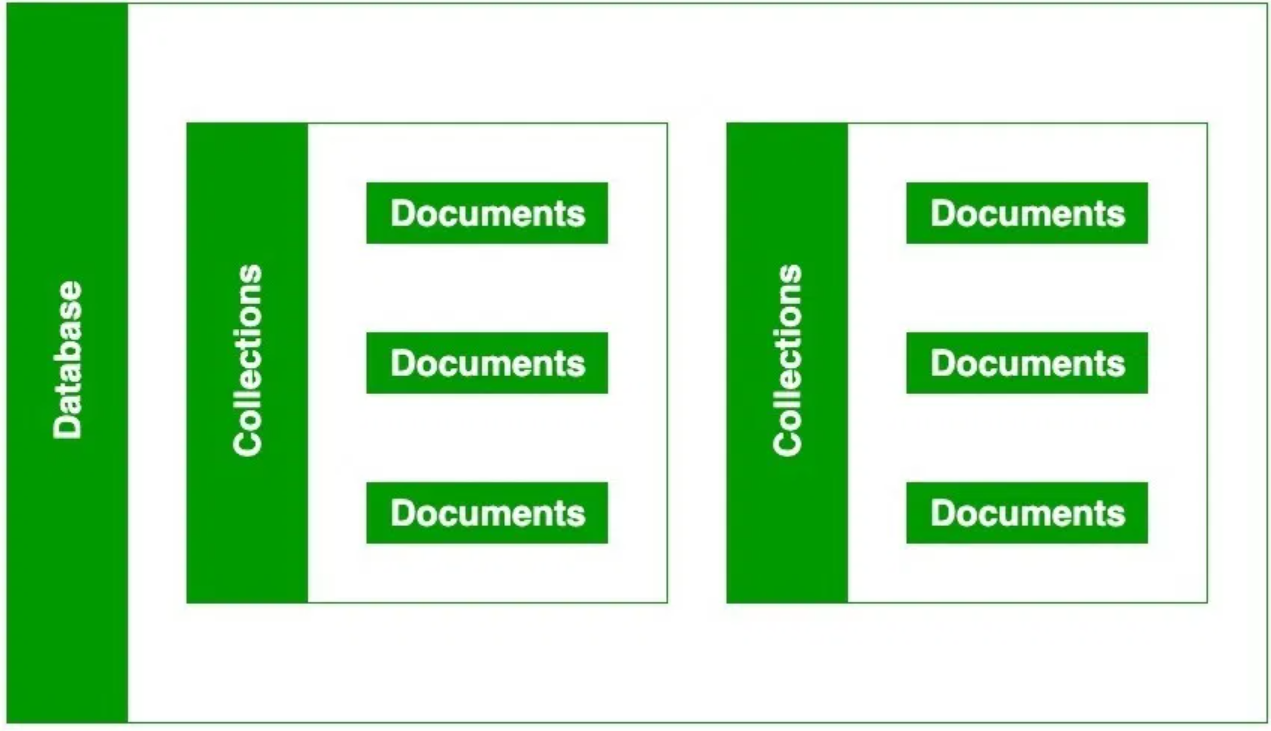
\includegraphics[width=0.7\linewidth]{img/mongoDB/HD_db.png}
        \caption{Cách hoạt động của MongoDB. Nguồn \cite{noauthor_mongodb--gi-1jpeg_nodate}}
        \label{fig:web_scraping}
    \end{figure}
    
    \begin{itemize}[left=0.5cm] 
        \item[$\bullet$] Cơ sở dữ liệu MongoDB lưu trữ tài liệu trong các collections, tương tự như bảng trong cơ sở dữ liệu quan hệ. Mỗi collection có thể chứa nhiều tài liệu (documents) có cấu trúc dữ liệu tùy ý.         
        \item[$\bullet$]Bây giờ bên trong collection sẽ có tài liệu (documents). Các tài liệu này sẽ chứa dữ liệu mà bạn muốn lưu trữ trong MongoDB database. Mỗi document có thể chứa nhiều fields dữ liệu, mỗi field được định danh bằng tên và có giá trị tương ứng.
        \newpage
        
        \item[$\bullet$]Các tài liệu (documents) được tạo bằng cách sử dụng các field. Các field là các key-value pair trong tài liệu, nó giống như các cột trong cơ sở dữ liệu quan hệ. Giá trị của fields có thể thuộc bất kỳ loại dữ liệu BSON nào như double, string, boolean,...
        
        \item[$\bullet$]MongoDB hỗ trợ việc tạo index cho các field dữ liệu trong collection, giúp tăng tốc độ truy vấn. Chúng còn hỗ trợ sao chép dữ liệu giữa các node trong một cluster giúp đảm bảo tính khả dụng và độ tin cậy của hệ thống.
        
        \item[$\bullet$]MongoDB phân tán dữ liệu trên nhiều node, giúp tăng khả năng mở rộng của hệ thống, đồng thời chúng còn hỗ trợ tính toán phân tán bằng cách sử dụng MapReduce giúp xử lý dữ liệu lớn một cách hiệu quả.   
    \end{itemize}
    
    \item []\hspace*{0.7cm}Khi sử dụng MongoDB, bạn có thể sử dụng API và driver của MongoDB để truy cập và thao tác với dữ liệu trong hệ thống cơ sở dữ liệu này.\cite{noauthor_mongodb_2023_text}
\end{enumerate}


\subsection{Ưu điểm và hạn chế}
\begin{enumerate}
    \item []\textbf{Ưu điểm:}
    \begin{itemize}[left=0.5cm] 
        \item[-] \textbf{Khả năng mở rộng và linh hoạt:}  MongoDB mở rộng tốt, xử lý dữ liệu lớn và dễ dàng mở rộng theo chiều ngang. Thiết kế lược đồ linh hoạt giúp điều chỉnh nhanh chóng cho ứng dụng phát triển nhanh.
        
        \item[-] \textbf{Hiệu suất và tốc độ:} MongoDB tối ưu hóa cho đọc và ghi với thông lượng cao, lý tưởng cho ứng dụng cần xử lý dữ liệu nhanh, nhờ vào lập chỉ mục, sao chép và sharding.
        
        \item[-]\textbf{Ngôn ngữ truy vấn phong phú:} Ngôn ngữ truy vấn mạnh mẽ cho phép thực hiện các truy vấn phức tạp và biến đổi dữ liệu dễ dàng, nâng cao khả năng phân tích.
        
        \item[-] \textbf{Tài liệu giống như JSON:} Việc sử dụng BSON cho phép biểu diễn mối quan hệ phân cấp phức tạp, tích hợp tốt với ứng dụng web hiện đại.

        \item[-]\textbf{Hỗ trợ dữ liệu không gian địa lý:} MongoDB hỗ trợ dữ liệu không gian địa lý, rất hữu ích cho ứng dụng dựa trên vị trí như lập bản đồ và truy vấn không gian.

        \item[-]\textbf{Cộng đồng và hệ sinh thái mạnh mẽ:}  MongoDB có cộng đồng năng động và hệ sinh thái phong phú với nhiều công cụ, hỗ trợ phát triển ứng dụng.

    \end{itemize}
    \newpage

    \item [] \textbf{Hạn chế:}
    \begin{itemize}[left=0.5cm] 
        \item[-] \textbf{Sử dụng bộ nhớ:} Định dạng BSON của MongoDB có thể tiêu tốn nhiều bộ nhớ hơn so với các định dạng lưu trữ khác, gây bất lợi cho những ứng dụng có tài nguyên hạn chế.

        \item[-] \textbf{Giao dịch phức tạp:} Dù hỗ trợ giao dịch ACID đa tài liệu, nhưng tính năng này trong MongoDB còn khá mới và có thể chưa hoàn thiện như trong các hệ quản trị cơ sở dữ liệu quan hệ truyền thống.

        \item[-] \textbf{Vấn đề về tính nhất quán:} MongoDB thiết kế với tính nhất quán cuối cùng, điều này có thể không phù hợp cho các ứng dụng đòi hỏi tính nhất quán mạnh mẽ và chính xác tức thời.

        \item[-] \textbf{Giới hạn lập chỉ mục:} Một số loại cấu trúc dữ liệu và truy vấn có thể không được lập chỉ mục hiệu quả, gây ảnh hưởng đến hiệu suất.

    \end{itemize}
\end{enumerate}
\subsection{Các tính năng nổi bật của MongoDB}
\begin{enumerate}
    \item []
    \begin{itemize}[left=0.5cm]
    \item[$\bullet$]\textbf{Định hướng tài liệu:} MongoDB lưu trữ dữ liệu dưới dạng tài liệu với cặp khóa-giá trị, giúp tăng tính linh hoạt so với các bảng trong RDBMS. Mỗi tài liệu có một ID duy nhất.
    
    \item[$\bullet$]\textbf{Cơ sở dữ liệu không có lược đồ:} MongoDB cho phép một bộ sưu tập chứa nhiều loại tài liệu khác nhau mà không yêu cầu phải có cấu trúc giống nhau, mang lại tính linh hoạt cao.

    \item[$\bullet$] \textbf{Khả năng mở rộng:} MongoDB hỗ trợ mở rộng theo chiều ngang thông qua sharding, cho phép phân phối dữ liệu trên nhiều máy chủ, giúp dễ dàng thêm máy mới vào hệ thống.

    \item[$\bullet$] \textbf{Lập chỉ mục:} MongoDB tự động lập chỉ mục mọi trường trong tài liệu, giúp tăng tốc độ truy xuất và tìm kiếm dữ liệu so với việc tìm kiếm từng tài liệu không được lập chỉ mục.

    \item[$\bullet$]\textbf{Tổng hợp:} MongoDB hỗ trợ thực hiện các phép toán tổng hợp trên dữ liệu với ba phương pháp: ống tổng hợp, chức năng giảm ánh xạ, và tổng hợp đơn mục đích.

    \item[$\bullet$]\textbf{Hiệu suất cao:} Với các tính năng như mở rộng, lập chỉ mục và sao chép, MongoDB có hiệu suất cao và độ bền dữ liệu vượt trội so với các cơ sở dữ liệu khác.\cite{noauthor_top_2021_features_db}
\end{itemize}
\end{enumerate}
\newpage
\begin{enumerate}
    \item []

\end{enumerate}
\subsection{So sánh MongoDB và RDBMS}
\begin{enumerate}
    \item []
    \begin{itemize}[left=0.7cm]
        \item[]1.Cấu trúc dữ liệu:
        \begin{itemize}[left=0.5cm]
             \item [$\bullet$]\textbf{MongoDB:} Lưu trữ dữ liệu dưới dạng tài liệu JSON (BSON), cho phép linh hoạt trong cấu trúc và kiểu dữ liệu.
             \item [$\bullet$]\textbf{RDBMS:} Sử dụng bảng với các hàng và cột có cấu trúc cố định.
        \end{itemize}
        \item[] 
        \item[]2.Tính mở rộng:
        \begin{itemize}[left=0.5cm]
             \item [$\bullet$]\textbf{MongoDB:} Mở rộng ngang (sharding).
             \item [$\bullet$]\textbf{RDBMS:} Thường mở rộng dọc (vertical scaling).
        \end{itemize}
        \item[] 
        \item[]3.Khả năng xử lý giao dịch:
        \begin{itemize}[left=0.5cm]
             \item [$\bullet$]\textbf{MongoDB:} Hỗ trợ giao dịch tài liệu.
             \item [$\bullet$]\textbf{RDBMS:} Tính năng ACID\footnote{
ACID là các thuộc tính đảm bảo tính toàn vẹn giao dịch trong cơ sở dữ liệu: Atomicity (giao dịch hoàn thành toàn bộ hoặc không), Consistency (dữ liệu luôn ở trạng thái hợp lệ), Isolation (giao dịch hoạt động độc lập), và Durability (thay đổi được lưu trữ vĩnh viễn sau khi hoàn tất).} mạnh mẽ.
        \end{itemize}
        \item[] 
        \item[]4.Truy vấn dữ liệu:
        \begin{itemize}[left=0.5cm]
             \item [$\bullet$]\textbf{MongoDB:} Ngôn ngữ truy vấn linh hoạt.
             \item [$\bullet$]\textbf{RDBMS:} Ngôn ngữ SQL chuẩn.
        \end{itemize}
        \item[] 
        \item[]5.Mục đích sử dụng:
        \begin{itemize}[left=0.5cm]
             \item [$\bullet$]\textbf{MongoDB:} Dữ liệu phi cấu trúc, ứng dụng web.
             \item [$\bullet$]\textbf{RDBMS:} Tính toàn vẹn dữ liệu cao, ứng dụng tài chính.\cite{noauthor_difference_2019}
        \end{itemize}
    \end{itemize}


\end{enumerate}
\newpage
\subsection{Công cụ hỗ trợ MongoDB}
\begin{enumerate}
    \item [] \hspace*{0.7cm}MongoDB có nhiều công cụ hỗ trợ giúp người dùng dễ dàng quản lý và làm việc với cơ sở dữ liệu. Hai công cụ phổ biến nhất là Robo 3T và MongoDB Compass.\cite{noauthor_mongodb_nodate_support}
    \begin{itemize}[left= 0.7cm]
        \item [$\bullet$]\textbf{Robo 3T}(trước đây là Robomongo) là một công cụ miễn phí mã nguồn mở, cung cấp giao diện đồ họa thân thiện giúp người dùng tương tác với MongoDB. Nó hỗ trợ các chức năng như kết nối, duyệt và chỉnh sửa cơ sở dữ liệu trực quan, phù hợp cho những người cần một công cụ đơn giản và nhẹ nhàng.

        \item [$\bullet$]\textbf{MongoDB Compass} là công cụ chính thức do MongoDB phát triển. Đây là một ứng dụng GUI (Giao diện người dùng đồ họa) đầy đủ tính năng, cho phép người dùng không chỉ duyệt và chỉnh sửa dữ liệu mà còn phân tích hiệu suất truy vấn và tối ưu hóa cấu trúc cơ sở dữ liệu. Ngoài ra, Compass còn cung cấp khả năng hiển thị trực quan về dạng dữ liệu và mối quan hệ giữa các đối tượng trong MongoDB, hỗ trợ người dùng trong việc kiểm tra và xác thực dữ liệu.
    \end{itemize}
    
\end{enumerate}
\begin{enumerate}
    \item []
    \item[]
     
\end{enumerate}
\subsection{Cách thức thao tác với MongoDB} 
\begin{enumerate}
    \item []\hspace*{0.3cm}\textbf{1. Cài Đặt MongoDB}
    \begin{itemize}[left = 0.5cm]
        \item []MongoDB có thể cài đặt trên Windows, macOS và Linux. Người dùng tải bản cài đặt từ trang chủ MongoDB và làm theo hướng dẫn. Sau khi cài đặt, có thể cấu hình MongoDB chạy tự động khi khởi động hệ thống.
    \end{itemize}
    \item[] 
    \item []\hspace*{0.3cm}\textbf{2. Kết Nối Tới MongoDB}
    \begin{itemize}[left = 0.5cm]
        \item [$\bullet$]MongoDB Shell (mongosh): Sử dụng lệnh mongosh trong terminal để quản lý và thao tác với cơ sở dữ liệu.

        \item [$\bullet$]Kết Nối Từ Ứng Dụng: Kết nối qua các ngôn ngữ lập trình như Python (thư viện pymongo) hoặc Node.js (thư viện mongodb) để tương tác với cơ sở dữ liệu.
    \end{itemize}
    \newpage
    \item[] 
    \item []\hspace*{0.3cm}\textbf{3. Tạo Cơ Sở Dữ Liệu}
    \begin{itemize}[left = 0.5cm]
        \item []Trong Trong MongoDB, không cần lệnh riêng để tạo cơ sở dữ liệu; khi người dùng thêm dữ liệu vào cơ sở dữ liệu chưa tồn tại, MongoDB sẽ tự động tạo nó. Để chọn hoặc tạo cơ sở dữ liệu mới, sử dụng lệnh:
        \begin{center}
            \textbf{use database\_name}
        \end{center}
         \item []Lệnh này sẽ chuyển đến cơ sở dữ liệu database\_name và tự động tạo nếu nó chưa tồn tại.
        
    \end{itemize}
    \item[]
     
    \item []\hspace*{0.3cm}\textbf{4. Tạo Collection}
    \begin{itemize}[left = 0.5cm]
        \item []Collection trong MongoDB lưu trữ các tài liệu. Người dùng có thể tạo Collection bằng lệnh:
        \begin{center}
            \textbf{db.createCollection("collection\_name")}
        \end{center}
         \item []Tuy nhiên, Collection cũng sẽ tự động được tạo khi người dùng chèn dữ liệu vào.
    \end{itemize}
    \item[] 
    \item []\hspace*{0.3cm}\textbf{5. Chèn Dữ Liệu}
    \begin{itemize}[left = 0.5cm]
        \item []Dữ liệu trong MongoDB được lưu trữ dưới dạng tài liệu BSON. Để chèn tài liệu vào Collection, sử dụng lệnh:
         \begin{center}
            \textbf{db.collection\_name.insert({name: "Linh", age: 20})}
        \end{center}
        \item []Lệnh này sẽ lưu thông tin của một người tên "Linh" và tuổi 20.
    \end{itemize}
    \item[] 
    \item []\hspace*{0.3cm}\textbf{6. Truy Vấn Dữ Liệu}
    \begin{itemize}[left = 0.5cm]
        \item []MongoDB cho phép truy vấn dữ liệu với nhiều điều kiện khác nhau. Sử dụng lệnh find() để tìm kiếm:
         \begin{center}
            \textbf{db.collection\_name.find({name: "Linh"})}
        \end{center}
        \item []Lệnh trên sẽ trả về tất cả các tài liệu có trường name là "Linh".
    \end{itemize}
    \newpage
    \item[]
    
    \item []\hspace*{0.3cm}\textbf{7. Cập Nhật Dữ Liệu}
    \begin{itemize}[left = 0.5cm]
        \item []Người dùng có thể cập nhật tài liệu bằng lệnh \textit{updateOne()} hoặc \textit{updateMany()}:
         \begin{center}
            \textbf{db.collection\_name.updateOne({name: "Linh"}, {\$set: {age: 22}})
}
        \end{center}
        \item []Lệnh này sẽ cập nhật tuổi của "Linh" thành 22.


    \end{itemize}
    \item[] 
    \item []\hspace*{0.3cm}\textbf{8. Xóa Dữ Liệu
}
    \begin{itemize}[left = 0.5cm]
        \item []Để xóa dữ liệu, sử dụng lệnh \textit{deleteOne()} hoặc \textit{deleteMany()}:
         \begin{center}
            \textbf{db.collection\_name.deleteOne({name: "Linh"})}
        \end{center}
        \item []Lệnh này sẽ xóa tài liệu có tên "Linh" trong Collection.\cite{noauthor_how_nodate}
    \end{itemize}
\end{enumerate}
